\section{eo\-Eval\-Continue$<$ EOT $>$ Class Template Reference}
\label{classeo_eval_continue}\index{eoEvalContinue@{eoEvalContinue}}
Continues until a number of evaluations has been made.  


{\tt \#include $<$eo\-Eval\-Continue.h$>$}

Inheritance diagram for eo\-Eval\-Continue$<$ EOT $>$::\begin{figure}[H]
\begin{center}
\leavevmode
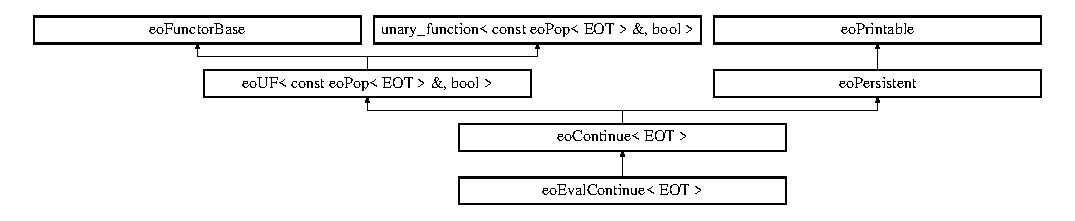
\includegraphics[height=2.52252cm]{classeo_eval_continue}
\end{center}
\end{figure}
\subsection*{Public Member Functions}
\begin{CompactItemize}
\item 
{\bf eo\-Eval\-Continue} ({\bf eo\-Eval\-Func\-Counter}$<$ {\bf EOT} $>$ \&\_\-eval, unsigned long \_\-total\-Eval)\label{classeo_eval_continue_a0}

\begin{CompactList}\small\item\em Ctor. \item\end{CompactList}\item 
virtual bool {\bf operator()} (const {\bf eo\-Pop}$<$ {\bf EOT} $>$ \&\_\-v\-EO)\label{classeo_eval_continue_a1}

\begin{CompactList}\small\item\em Returns false when a certain number of evaluations has been done. \item\end{CompactList}\item 
virtual unsigned long {\bf total\-Evaluations} ()\label{classeo_eval_continue_a2}

\begin{CompactList}\small\item\em Returns the number of generations to reach. \item\end{CompactList}\item 
virtual std::string {\bf class\-Name} (void) const \label{classeo_eval_continue_a3}

\end{CompactItemize}
\subsection*{Private Attributes}
\begin{CompactItemize}
\item 
{\bf eo\-Eval\-Func\-Counter}$<$ {\bf EOT} $>$ \& {\bf eval}\label{classeo_eval_continue_r0}

\item 
unsigned long {\bf rep\-Total\-Evaluations}\label{classeo_eval_continue_r1}

\end{CompactItemize}


\subsection{Detailed Description}
\subsubsection*{template$<$class EOT$>$ class eo\-Eval\-Continue$<$ EOT $>$}

Continues until a number of evaluations has been made. 



Definition at line 36 of file eo\-Eval\-Continue.h.

The documentation for this class was generated from the following file:\begin{CompactItemize}
\item 
eo\-Eval\-Continue.h\end{CompactItemize}
